\documentclass[pdftex,12pt,letter]{article}
\usepackage[pdftex]{graphicx}

\usepackage{pdfpages} 
\usepackage{fixltx2e}

\addtolength{\textwidth}{3.5cm}
\addtolength{\hoffset}{-2cm}
\addtolength{\textheight}{4.5cm}
\addtolength{\voffset}{-3cm}

\bibliographystyle{plain}
\usepackage{natbib}
\newcommand{\HRule}{\rule{\linewidth}{0.5mm}}

\renewcommand{\thesection}{\Alph{section}}

%\usepackage{blindtext}
\usepackage{listings}

\usepackage{amsmath}

\usepackage{subfig}
\begin{document}
\begin{titlepage}

\begin{center}


% Upper part of the page

\includegraphics[width=.5\textwidth]{./logo}\\[1cm]    

\textsc{\LARGE CS-GY 6903: Modern Cryptography}\\[1.5cm]

\textsc{\Large Professor: Giovanni Di Crescenzo}\\[0.5cm]

% Title
\HRule \\[0.4cm]
{ \large \bfseries Project 1:\\
{\small Breaking Polyalphabetic ciphers}}\\[0.4cm]

\HRule \\[1.5cm]
% first column
\begin{minipage}{0.4\textwidth}
\begin{flushleft}
\large Santiago Torres-Arias\\
{\small {\bf NYU ID: N14553751 } }
\end{flushleft}
\end{minipage}
%second column
\begin{minipage}{0.40\textwidth}
\begin{flushright}
\large Lucas Mladek\\
{\small {\bf NYU ID: N1xxxxxx } } 
\end{flushright}
\end{minipage} 

\vfill

% Bottom of the page
{\large \today}

\end{center}
\end{titlepage}

\newpage
\tableofcontents
\newpage

\section{Introduction}

Polyalphabetic ciphers have been around in humanity for hundreds of years now.
And, although their use is no longer recommended for serious cryptography, its
use is still widespread among cryptography amateurs and cryptography
challenges.

It is known that polyalphabetic ciphers are subject to frequency analysis, and
known plaintext attacks. The focus of this writeup is to introduce techniques
that leverage this knowledge to break these ciphers in the least possible time.

\section{Understanding polyalphabetic ciphers}
% Here, we talk about what's a polyalphabetic cipher
% and how the guy must be high about thinking of the j(x) function


\subsection{The anatomy of the $j(i)$ function}

We can try to decompose the $j(i)$ function by using calculus concepts. The
following equation provides a simplified version of the possible variants that
$j(i)$ can have:

\begin{equation}
    j(i) = \left( \frac{xi^y}{z} + m \right) \mod{t}
\end{equation}

In this equation, we adopt the following nomenclature:
\begin{itemize}
    \item i is the index
    \item x is a define a ``decimating coefficient'' for i.
    \item y defines a ``decimating exponential'' factor for the index. (we
        assume y = 1 for simplicity)
    \item The constant term $z$ defines a ``stretching factor''
    \item m is a ``start offset'', and it can be described as shifting the key
        by m bins.
    \item $\mod{t}$ guarantees that the values selected are inside the
        generated key and t is the length of the key.
    \item we assume $\frac{x}{z}$ is a multiple of t, this makes it periodic on t.
\end{itemize}

The relationship between the upper and lower factors define how this function
behaves.  In general, we can consider to be three variants: periodic,
decimating and stretching. 

\subsection{Key stretching and key-decimating}

When the factor above ($x$) is bigger than the factor below ($z$), then we can
assume that we have a key-decimating function. Key decimating functions make
the key essentially "smaller" in a sense that some values are skipped and hence
lost (depending on the periodicity).

On the other hand, when values from the upper monomial are smaller than the
lower one, we have what's called a key-stretching function. When this happens,
we see that -- due to integer math -- some values are repeated contiguously.
For example, imagine that we have the following $j(i)$:

\begin{equation}
    j(i) = \frac{i}{4}\mod{30}
\end{equation}

In this case, the resulting function can be considered stretching because
values for i below 4 will all point to the element 0 in the original key.

For key-stretching functions, we will be unable to decrypt the ciphertext with the
provided code. However, some methods allow for guesswork on resulting decryption
attempts to figure out whether the function is stretching or not (in other words, if
the key we are obtaining seems to be repeated over and over our attack could leverage
this information to further decrypt stretching functions).

For key-decimating functions, we will be able to decrypt the ciphertext if
$\frac{x}{z}$ is a factor of t and therefore periodic on t. When this
assumption holds, we would need to search for the ``true'' period of the
ciphertext by variating this factor over and over.

The nature of this equation has a direct effect on what we will call the key's
periodicity.

\subsection{Periodicity}

Periodicity of the key (and $j(i)$) can be understood as ``the number of values for i
before the key-selecting sequence repeats''. Understanding this can allow us for 
an easy definition of a break function. 

We will define 'regular periodic functions' as those functions in which
$\frac{x}{z} \leq t$ and is also a multiple of t. When this happens, the
periodicity of $j(i)$ also falls in a multiple of t. For our breaking scheme,
we considered the function $j(i)$ to  be a regular periodic function since it
was the easiest to analyze. 

However, we could break Non-regular periodic functions by finding the same
subset of the key in different places along the ciphertext. This is a regular
step in breaking polyalphabetic cihpers if you are not given the key length.
Since we were given the key length we did not take this approach.   

\subsection{Why periodicity matters and $j(i)$ not as much}

If we consider a function to be regular periodic, then we can assume that the
set of keys from ${a...z}^t$ mapped under a specific $j(i)$ is only a different
permutation of the same set of keys under a different $j(i)$. In other words,
for both produced sets (from $j(i) and j'(i)$) there exists a large number of
``equivalent keys''.Knowing this, we can assume that, when a function is
regular periodic, obtaining a proposed key for $j(i) = i \mod(t)$ is a safe
bet. We will use this assumption in our breaking mechanisms, as it simplifies
our analysis greatly. Refer to figure~\ref{key-sets} for a graphic description
of this.

\begin{figure}[ht!]
    \centering
    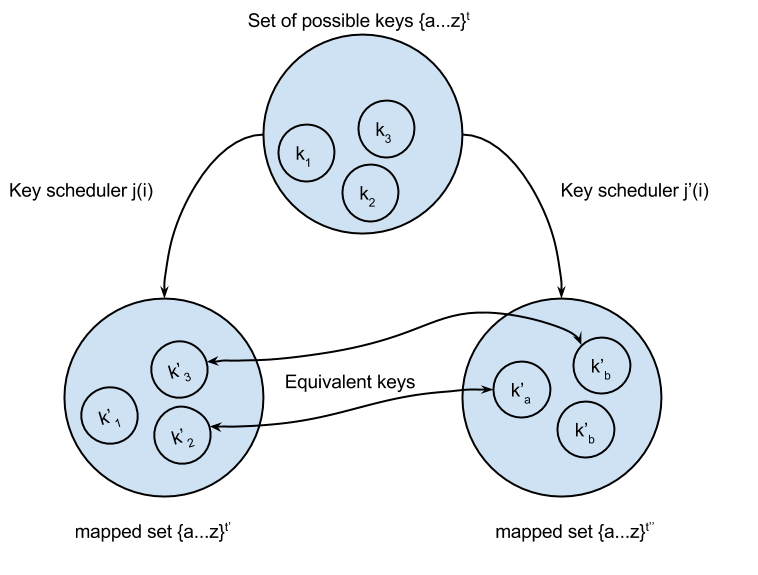
\includegraphics[width=.8\textwidth]{key-mapping}
    \caption{Different sets are mapped using different functions $j(i)$ but,
    if $j(i)$ and $j'(i)$ share periods, both sets will share a large amount of keys.}
    \label{key-sets}
\end{figure}

\subsection{Frequency analysis on polyalphabetic ciphers}

In most cases frequency analysis breaks polyalphabetic cihpers. However,
for this project the cihper text we are able to sample is too small to 
perform frequency analysis successfully. 

Kasiski Examination is another technique that would work and is similar to 
a frequency analysis but also requires us to be able to sample a greater amount 
of ciphertext to find words encrypted with the same portion of the key.

However, we know that, given the properties of the ciphertexts. We must, at least,
have two periods of the ciphertexts encrypted with the same portion of the key. This
becomes obvious since the maximum value for t is 40 (with 2t being 80) and L being at
least 100. This allows for variations of known-plaintext-attack.

\section{Breaking dictionary 1}

In order to design the most efficient mechanism to break the defined cipher, we 
first need to understand the nature of the existing dictionaries. In this case
we know that the existing plaintexts falls in a range of 150 different plaintexts
so we decided to analyse them as words.

This is known as a 'known plaintext attack'. The dictionaries given were a small 
enough set to be analyzed using the methods outlined in this section. 

\subsection{Minimum prefix: plaintexts as words}

Since the set of possible messages from Dictionary one is the same as the
number of entries a dictionary 1, cryptanalysis is really easy. We could
consider that the messages from dictionary one are a single, long word
encrypted and sent through the wire.

To understand this, we build a python script called "minimum\_prefix.py",
\footnote{ we provide this script as part of the supporting code under the
scripts subdirectory} that analyses the words in a dictionary to identify the
minimum amount of characters needed to differentiate plaintext from each other.
The result of this script outputs a value of 9 for Dictionary 1\footnote{we
tried to use the same approach for dictionary two but there is no minimum
prefix for it}, and we used it as part of our dictionary-header definition.

We can obtain a possible, equivalent key by substracting a piece of plaintext from the
ciphertext:

\begin{equation}
    p_{[i]} + k_{[x]} = c_{[i]} \rightarrow k_{[x]} = c_{[i]} - p_{[i]}
\end{equation}

Now, how do we know our proposed key is correct?

\subsection{Defining our Oracle and Attack}

Breaking dictionary 1 is easy: we only need to apply the prefix plaintext to
the provided ciphertext and apply the resulting  key to another portion of
the ciphertext. The only catch is that we need to identify a region that uses
the same range of the key. Since we assumed $j(i)$ to be regular periodic, then
we can assume that $t$ is a place where period starts and verify if the result
matches correct plaintext of the same dictionary entry in that location. 

We used a few 'speed-ups' in our code, for example declaring the entire
dictionary as a constant in C, alphabetizing the the dictionary, and 
using a 'trampolining' function to jump the the first letter of the
alphabetized potential plaintext dictionary to speed up verification.  

The code we wrote for this takes less than a second to verify and dismiss all
possible candidates for the plaintext. 

\begin{figure}[ht!]
    \centering
    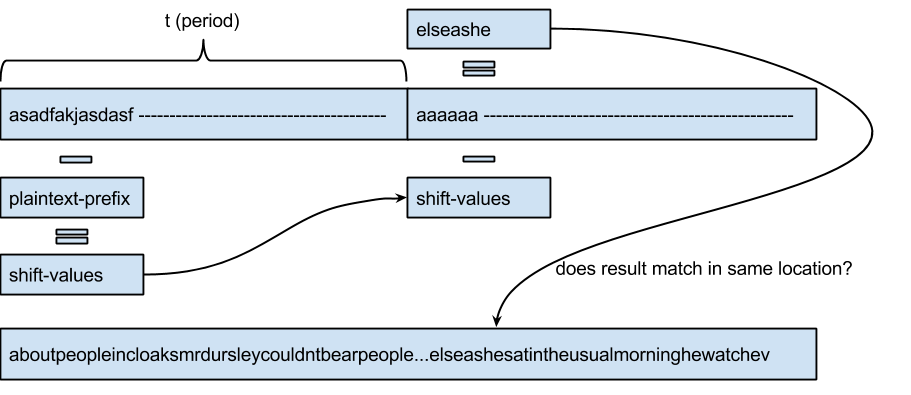
\includegraphics[width=.8\textwidth]{breaking-dict1}
    \caption{The breaking procedure from ciphertexts produced from Dictionary 1}
    \label{breaking-dict1}
\end{figure}

\section{Breaking dictionary 2}

For dictionary 2 we can't use the same exact method as dictionary 1.
So we researched different possible methods and case studies that were 
relevant to our attack. Before we explain our attack we will give a 
brief explanation of one such case study that help formulate our attack
strategy.  

\subsection{Case study: Rosignol Cipher - The man with the Iron mask}

The Rosignol's were a family of French cryptographers in the 17th
century\footnote{ https://en.wikipedia.org/wiki/Great\_Cipher} .  The most
famous of the family was Antoine Rossignol and his son Bonaventure who in ~1626
developed a cryptographic code so strong it baffled cryptanalysts for centuries
(it wasn't decoded until 1893). This cipher used numbers to represent syllables
rather than individual characters (the common approach at that time).  The
technical nature of the cipher includes a small (587) set of numbers that
represent syllables and by itself is still subject to frequency analysis
attacks. 

In addition, this Cipher Schema seemed to pose a decryption/solution to solve the 
mystery of the man in the iron mask (infamous french prisoner at the time). 

This inspired the approach we took to cracking dictionary 2. We focused on 
tuples of characters (like syllables but not quite) and their possible combinations
in order to determine partials of words, or concatentations of 2 different words. 

\subsection{Breaking polyalphabetic ciphers using N-character tuples (trillables)}

\subsubsection{The size of the set}

The size of the set is important to note for breaking dictionary 2 using
tuples.  Set groups as we make tuples bigger grow, but the probability of them
appearing in the plaintext decreases. We found 3 tuples to be of an optimal
size for our purposes and thus have dubbed them triads or trillables. 

\subsubsection{Probabilistic results}

Every time we decrypt a 3-character tuple(trillable) there is a probability(of
$\approx$ .1907) that it belongs to the subset of all possible trillables
produced from Dictionary 2.

In addition, as the number of trials (in our case each trial is a decryption
attempt of a piece of ciphertext) increases, the probability that all of the
trillables fall into the subset of possible trillables decreases.  

Theoretically there are possible collisions that don't make this a fully
encompassing approach.  However, this method is much faster so we are trading
quality for performance in order to make our overall decryption as fast as
possible.

\subsection{Defining our Oracle and Attack} 

We perform the same attack as in dictionary 1, however our oracle has changed. 
We now use the 3-character tuples (trillables) approach as defined in section D.2.2 
 
\begin{figure}[ht!]
    \centering
    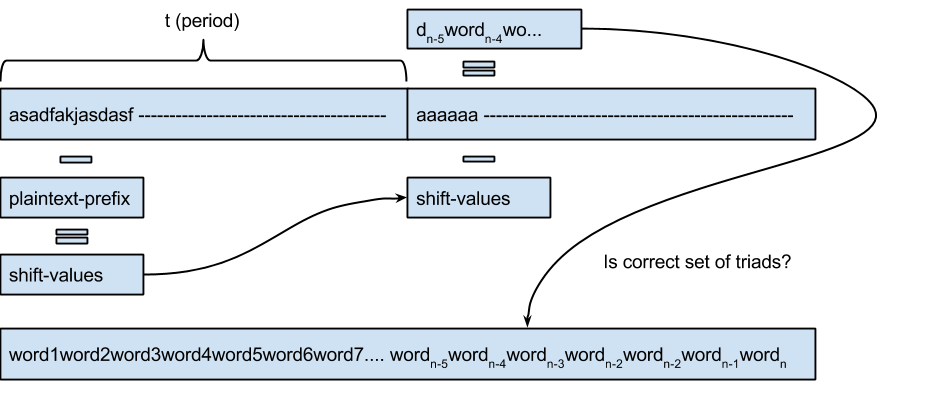
\includegraphics[width=.8\textwidth]{breaking-dict2}
    \caption{The breaking procedure from ciphertexts produced from Dictionary 2. Note
    how it's possible that the second decrypted subsection is part of a word, or even two or more
words}
    \label{breaking-dict1}
\end{figure}

We attempt to decrypt a piece of the ciphertext using a word in length $k$. We,
then, obtain a series of ``shifts'' (or equivalent key) and try to decrypt a
piece of ciphertext at length $t + k$.  From the obtained ``proposed
plaintext'' we verify if all the trillables belong to our valid subset. If it
does, then we move forward our value k until it overlaps or reaches t; every
time we decrypt a piece of ciphertext, we verify that all the trillables (even
between words) fall into the set.

If a trillable is not in this set, we move back in k and change the proposed
word. Once we have plaintext with all valid trillables, we verify that the whole
string only contains words from dictionary 2 as a last step. If this is
true, then we found a proper plaintext.


\section{Results}

We made a script that randomly selects a $j(i)$ with our constraints listed
above and encrypts a plaintext from either dictionary 1 or 2. We used the
results of this script to test our decryption program.\footnote{you can find
 this code under the scripts/ subdirectory in the source folder}

We utilized benchmarking functions and unit testing in our code for efficiency
and troubleshooting respectively. This also increased code correctness in edge
cases, and gave us confidence in the results.

We also implemented a stopwatch timer in order to stop decryption attempts if
our program began to run our of time. However our decryption schema/program
runs so quickly we never needed to utilize it. 

The software architechture also allows for plug-and-play break-functions. This
allows us to include as many different breaking approaches as desired. If time
allowed for further extensions of the algorithm, our architechture would have
supported it.

We found that our program can decrypt the ciphertext generated by our script in
an extremely short amount of time relative to the 2 minutes upper limit for the
assignment. Timing tests return less than a second for both types of ciphers.

Lastly, we found no collisions that break our attack schema although admittedly
they could indeed exist and would affect a small number of cases with
dictionary 2. 
 
\section{Conclusion}

We researched and found different and creative ways for breaking polyalphabetic
ciphers.  Some of which were implementable but not within the given time period
for the project.  Others were infeasible due to the dictionary being relatively
short. Our attacks greatly depended on the fact the the key length is known and
the plaintext was given beforehand (this was a clear invitation to perform a
known plaintext attack).

Both partners Santiago and Luke were involved in the following tasks: Outlining
and Testing  Attack Strategies, Software Engineering and Coding, Analysis of
Results, Write-Up and Final Analysis.

\end{document}
